\title{Giving Machines Memory and Focus:  Evaluating Attention-Based and Memory-Based Neural Network Models on Large Q\&A Datasets} 
\author{Dan Strawser}

\documentclass{article}

\usepackage{amsmath}
\usepackage{graphicx}
\usepackage{amsfonts}

\DeclareMathOperator*{\argmax}{\arg\!\max}

\begin{document}
\maketitle
\begin{abstract}
This is what the project is about
\end{abstract}

\section{Introduction}

Question Answering tasks are some of the most general in natural language processing.          

This project focuses on QA tasks where some type of attention and inference is required.  For example, to answer the question posed in Fig. \ref{Fig:MC_Test}, the algorithm must be able to find the relevant phrases and infer Sally's motivation.  

\begin{figure}[!ht]
\label{Fig:MC_Test}
  \centering
    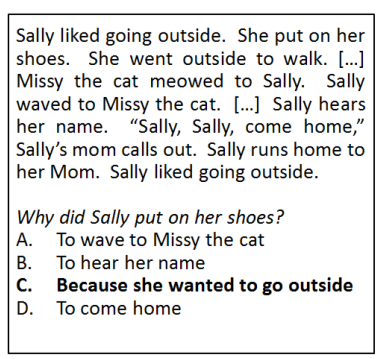
\includegraphics[width=0.3\textwidth]{images/mc_test}
      \caption{Example QA task from MC Test dataset.  Taken from \cite{karthik}.}    
\end{figure}

Many approaches have been proposed to solve this task, among them, feature-based methods.  Neural networks are another approach to solving this problem.  Recurrent neural networks seem especially well-suited for this problem because of their ability to use sequential data as input.  More recent models such as LSTM (Long Short Term Memory) units and GRU (Gated Recurrent Units) make it possible to train on longer sequences of data by avoiding the problem of exploding gradients.  However, some question and answer tasks require analyzing very large sequences of data and even these models have difficulty.  

Advancements made in the past year in deep neural networks provide more promise.  These networks combine the sequential encoding found in RNNs and add memory and attention.  Attention mechanisms are important because, given a large amount of information and a question, finding the relevant information is a challenge.  While these have shown promise on smaller corpora, it remains to be seen their advantages on larger datasets.  The goal of this project is to evaluate these neural network architectures and compare them against one another.  Specifically, I investigate the Memory Network described in \cite{Memory_Networks} and the Dynamic Memory Network from \cite{dmn}.

\section{Approaches}

\begin{figure}[!ht]
  \centering
    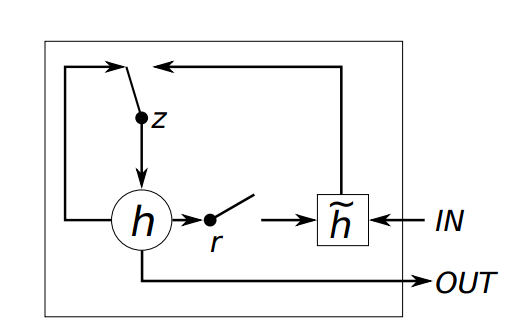
\includegraphics[width=0.4\textwidth]{images/GRU}
      \caption{Gated Recurrent Layer Architecture.  Taken from \cite{gru}.}    
\end{figure}


\begin{figure}[!ht]
\label{Fig:gru_encoder}
  \centering
    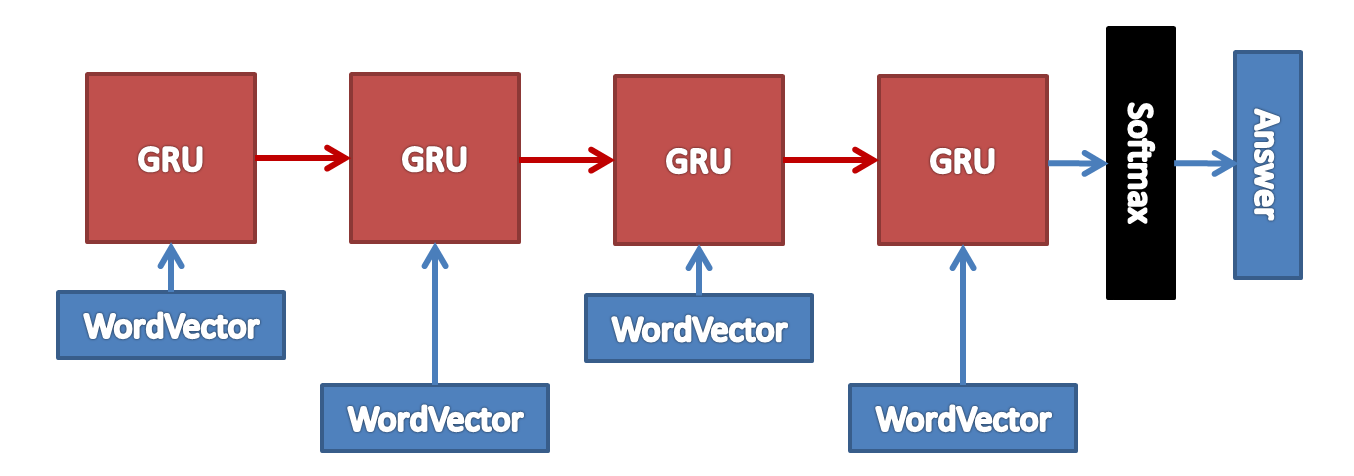
\includegraphics[width=0.8\textwidth]{images/GRU_encoder}
      \caption{Simple GRU Encoder.}    
\end{figure}


\subsection{GRU Encoder}

The baseline algorithm is simply a Gated Recurrent Unit (GRU) encoder, pictured in Fig. \ref{Fig:gru_encoder}.  This is simply a recurrent neural network that reads in each word of a sequence and, through a softmax layer, produces an output answer.  To form the sequence, a vector representing the question is concatenated with a vector containing the article (or information from which an answer is generated).  While the inputs can be generated by Word2Vec, for these experiments they were either one-hot vectors or word indices.  \par
The base unit for the Encoder (and also the subsequent Dynamic Memory Network) is the Gated Recurrent Unit.  The unit consists of two gates, a reset gate and an update gate, which determine whether or not to update the unit's hidden state with an input or simply propagate the previous hidden state.  

\subsection{Memory Network}

\begin{figure}
  \centering
    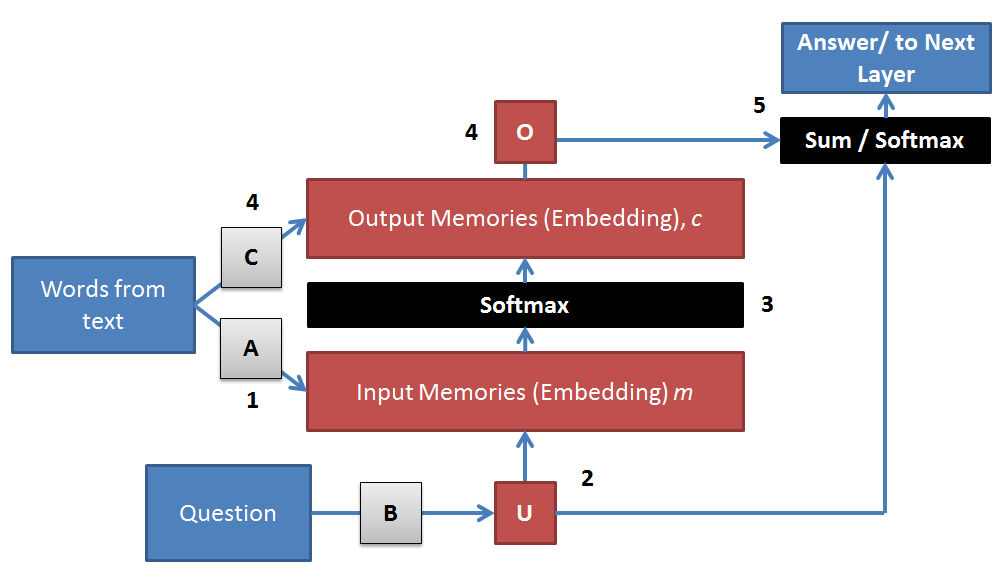
\includegraphics[width=1\textwidth]{images/mem_net}
      \caption{Memory Network Overview.}    
      \label{Fig:mem_net}      
\end{figure}

More recently, the Memory Network was described in \cite{mem_net} as an End-to-End algorithm.  This is important because it means that the algorithm only requires (\textit{text}, \textit{question}, \textit{answer}) tuples instead of relying on fact annotations.  The memory network is relatively simple in the fact that is relies on "memory" embeddings and softmax attention mechanisms. \par

For example, as described in \cite{mem_net}, an input sequence of words $W$ and an input question $Q$ are both transformed into embeddings through embedding matrices $A$ and $B$ respectively.  Question embeddings are transformed into "memory" embeddings $m$ (Numbered \textbf{1} in Fig. \ref{Fig:mem_net}) and questions into embeddings $b$ (Numbered \textbf{2} in Fig. \ref{Fig:mem_net}).  At this point a softmax layer is applied between the input and question embeddings (Numbered \textbf{3} in Fig. \ref{Fig:mem_net}): 
\begin{equation}
\label{Eq: softmax}
p_i = \text{Softmax} \left( u^Tm_i\right)
\end{equation}
Intuitively, this softmax determines which memories are relevant to answering the question.  In addition to the memory embeddings $m_i$, the input stream is also embed into an output embedding, $C$.  The result of the softmax layer, Eq. \ref{Eq: softmax}, is multiplied by this output embedding, Numbered \textbf{4}.  This result passes through a summation with the question state $u$, numbered \textbf{5}.  The result of the sum at \textbf{5} in Fig. \ref{Fig:mem_net} can either be passed to a softmax for a final answer or passed to another memory network layer.  That is, the layers are stacked and the result of one is passed to another as an input state $u$.  


\subsection{Dynamic Memory Network}

\begin{figure}
  \centering
    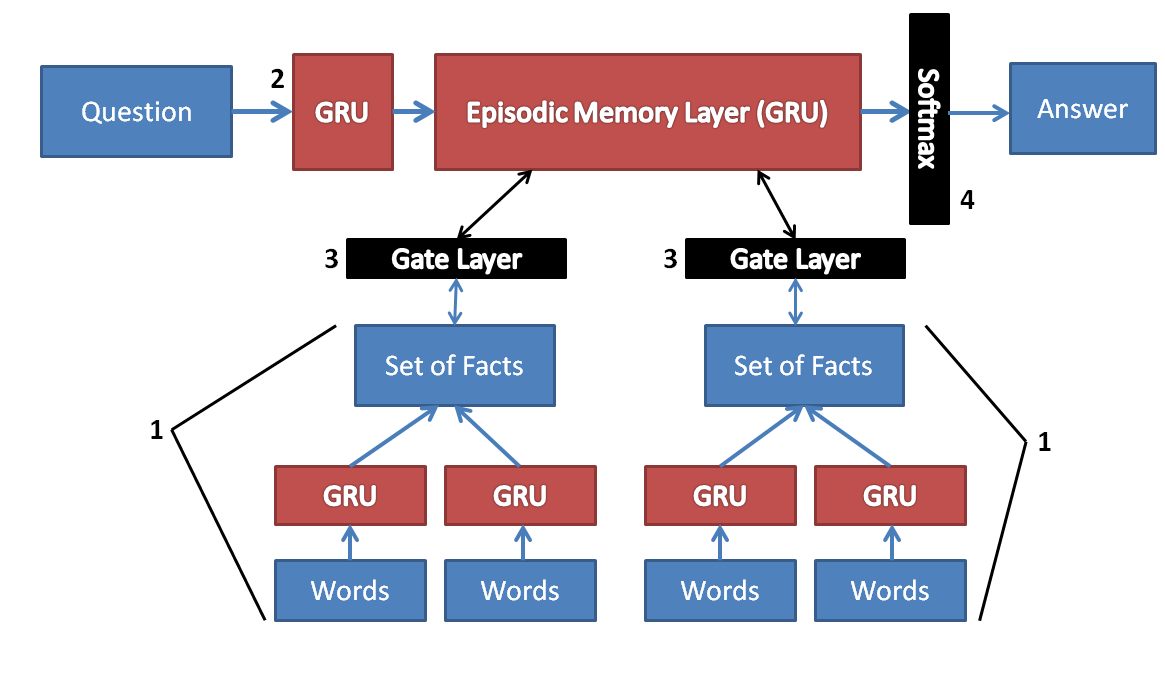
\includegraphics[width=1\textwidth]{images/dynam_mem_net}
      \caption{Dynamic Memory Network Overview.  The DMN shown represents a DMN that reads a document twice.}    
      \label{Fig:dmn}
\end{figure}

The final model investigated is the Dynamic Memory Network as presented in \cite{dmn}.  The dynamic memory network is somewhat similar to the Memory Network; however, it relies more explicitly on GRU encodings and adds the potential of "re-reading" sentences.  \par
First, each sentence is encoded into a fact through a GRU-based RNN.  This RNN reads each word in the sentence and updates its hidden state.  The final output, a "fact" encoding, is passed to the next layer.  This process is repeated for the entire document to generate a set of fact encodings, which is shown as \textbf{1} in Fig. \ref{Fig:dmn}.  \par
Next, given a set of facts from the entire document, it must be determined which of them is relevant to answering the given question.  For this, a gating mechanism is deployed, numbered \textbf{3}.  The functional form of this gate described in \cite{dmn} is: 
\begin{equation}
z\left( c_i, m, q \right) = \left[ c_i, m, q, c_i \circ q, c_i \circ m, \lvert c_i - q \rvert , \lvert c_i - m \rvert , c_i^T W^b q , c_i^T W^b m     \right] 
\end{equation}
\begin{equation}
g_i \left( c_i, m, q \right) = \sigma \left(W^a \text{tanh} \left(  W^c z \left(c_i, m,q \right)  \right)   \right) 
\end{equation}
where $c_i $ is the $i^{th}$ fact encoding, $m$ is the hidden state of the Episodic Layer (described below), and $q$ is the question encoding.  The magnitude of gate $g_i$ - a scalar - determines whether or not fact encoding $c_i$ will be passed to the episodic GRU-RNN.  This is done through a update equation:  
\begin{equation}
h_t = 1 = g_t \text{GRU} \left( c_t, h_{t-1} \right)  +  \left( 1 - g_t \right) h_{t-1} 
\end{equation}
The top episodic layer is used to read the facts and produce a final output.  \par One of the advantages of the DMN is that it can re-read a series of episodes.  This may be advantageous when the ordering of facts matters but when the second fact in the text occurred \textit{before} the first fact in the text, i.e. \textit{John went to the store on Saturday.  On the Wednesday prior, John drove to California.}.  Therefore, the example shown in Fig. \ref{Fig:dmn} is shown reading a document twice, producing two sets of facts, choosing episodes for each of these and then, finally, producing an output answer.   

\section{Datasets}

One of the challenges with QA tasks is designing datasets that are nontrivial and require inference to answer questions but are also large enough that the neural network will learn well.  

\subsection{Babi Tasks}

\begin{figure}
  \centering
    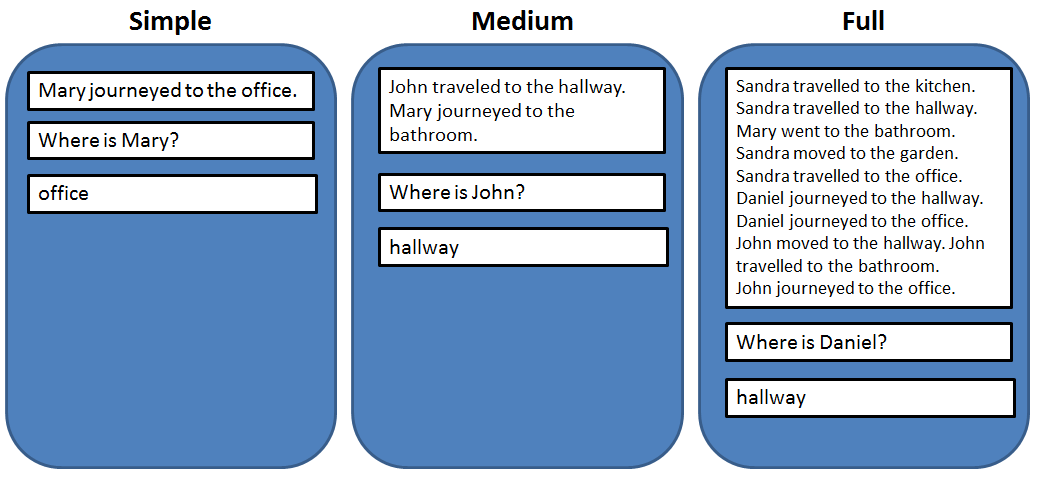
\includegraphics[width=1\textwidth]{images/babi_tasks}
      \caption{Examples of Babi tasks used for this project.}    
      \label{Fig:babi}
\end{figure}

The Babi Tasks are a set of 20 tasks created by researchers at Facebook and are described in .  The motivation is to create a set of tasks to test a general question answering algorithm.  The algorithm should be general in that it should be able to perform well on all of them and not just a few.  The set contains a wide variety of tasks.  For example, understanding orientation: \textit{The hallway is east of the bathroom.  The bedroom is west of the bathroom.  What is the bathroom east of?} or understanding counting objects: \textit{Mary moved to the bathroom. John went to the kitchen.  Mary took the football there.  How many object is Mary carrying?}.  \par
For this project, I focused on Babi Task 1, which involves determining where people went.  I split the task into simple, medium, and full versions as pictured in \ref{Fig:babi}.  The simple and medium were primarily for debugging - even the simple GRU encoder can easily obtain 100 \% correct responses on the simple version.    \par
An advantage of the Babi set is that it tests the neural networks on attention and inference.  However, their corpora is limited in size (Babi Task 1 only contains about 20 different words) and does not represent actual corpora that one may see in the real world.  

\subsection{WikiQA}

The second dataset that I used was one suggested by researchers at Carnegie Mellon involving Wikipedia article and questions that can be answered upon reading the article \cite{cmu}.  One example is shown in \ref{fig:wikiqa}.  An advantage of this dataset is that it represents a more realistic corpus size than the Babi Tasks.  However, a major disadvantage of the set is that it is very small.  It consists of approximately 200 articles and 5,000 questions concerning those articles.  As seen in the results, the neural networks have difficulty learning anything but basic yes/no questions on this dataset.  


\subsection{Google - CNN}

\begin{figure}[ht]
	\begin{minipage}[b]{0.45\linewidth}
		\centering
		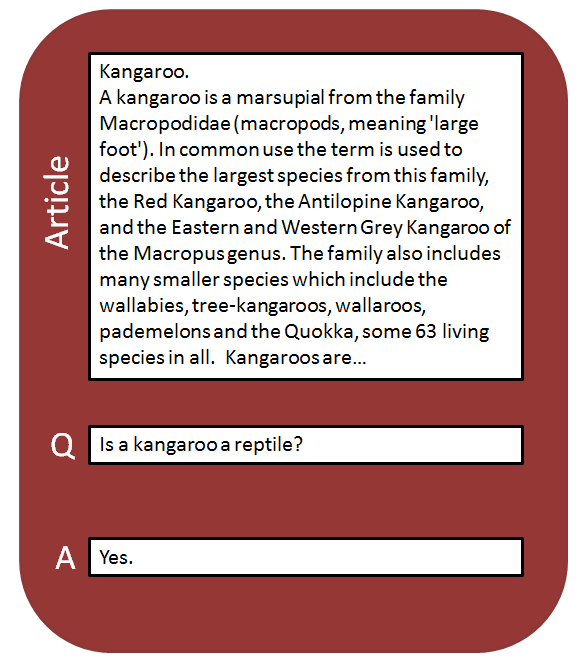
\includegraphics[width=\textwidth]{images/wikiqa}
		\caption{Example of article, question, and answer tuple from WikiQA dataset.  }
		\label{fig:wikiqa}
	\end{minipage}
	\hspace{0.5cm}
	\begin{minipage}[b]{0.45\linewidth}
		\centering
		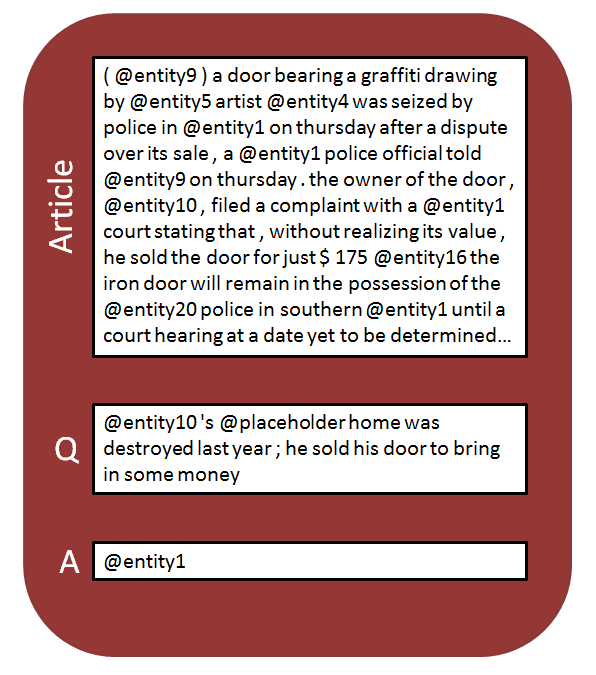
\includegraphics[width=\textwidth]{images/google_cnn}
		\caption{Example of Google-CNN article, question statement, and answer tuple.}
		\label{fig:google-cnn}
\end{minipage}
\end{figure}

The third dataset that I considered was provided by researchers at Google and described in \cite{goog_cnn}.  This dataset consists of articles from CNN (another similar dataset from Daily Mail is also described) with autonomously generated question statements and answers.  The question statements are generated through the simple, but effective, observation that all CNN/Daily Mail articles have accompanying human-written summaries.  Words can be replaced from these summaries to create question statements where an algorithm attempts to predict the word that was removed.  The advantage with creating training examples autonomously from a source like CNN is that a huge number can be produced (the full dataset is approximately one million articles).  While the WikiQA dataset has the problem of too few examples, this is not an issue with the CNN dataset.  

 







\nocite{*}
\bibliography{bibliography}
\bibliographystyle{IEEEtran}



\end{document}